% ==========================================
% BAB IV DESAIN KONSEP SOLUSI
% Memakai kolom tabel Y dan Z yang didefinisikan pada Bab III.
% Isi bab ini mengikuti Proposal_TA_Konten.docx (revisi 18 November 2026).
% ==========================================
\cleardoublepage % memastikan bab baru dimulai di halaman ganjil (kanan)
\chapter{DESAIN KONSEP SOLUSI}
\label{chap:desain-konsep-solusi}

% ============================================================================================
% IV.1 Gambaran umum
% ============================================================================================
\section{Gambaran Umum Rancangan}
\label{sec:gambaran-rancangan}

\begin{figure}[t]
  \centering
  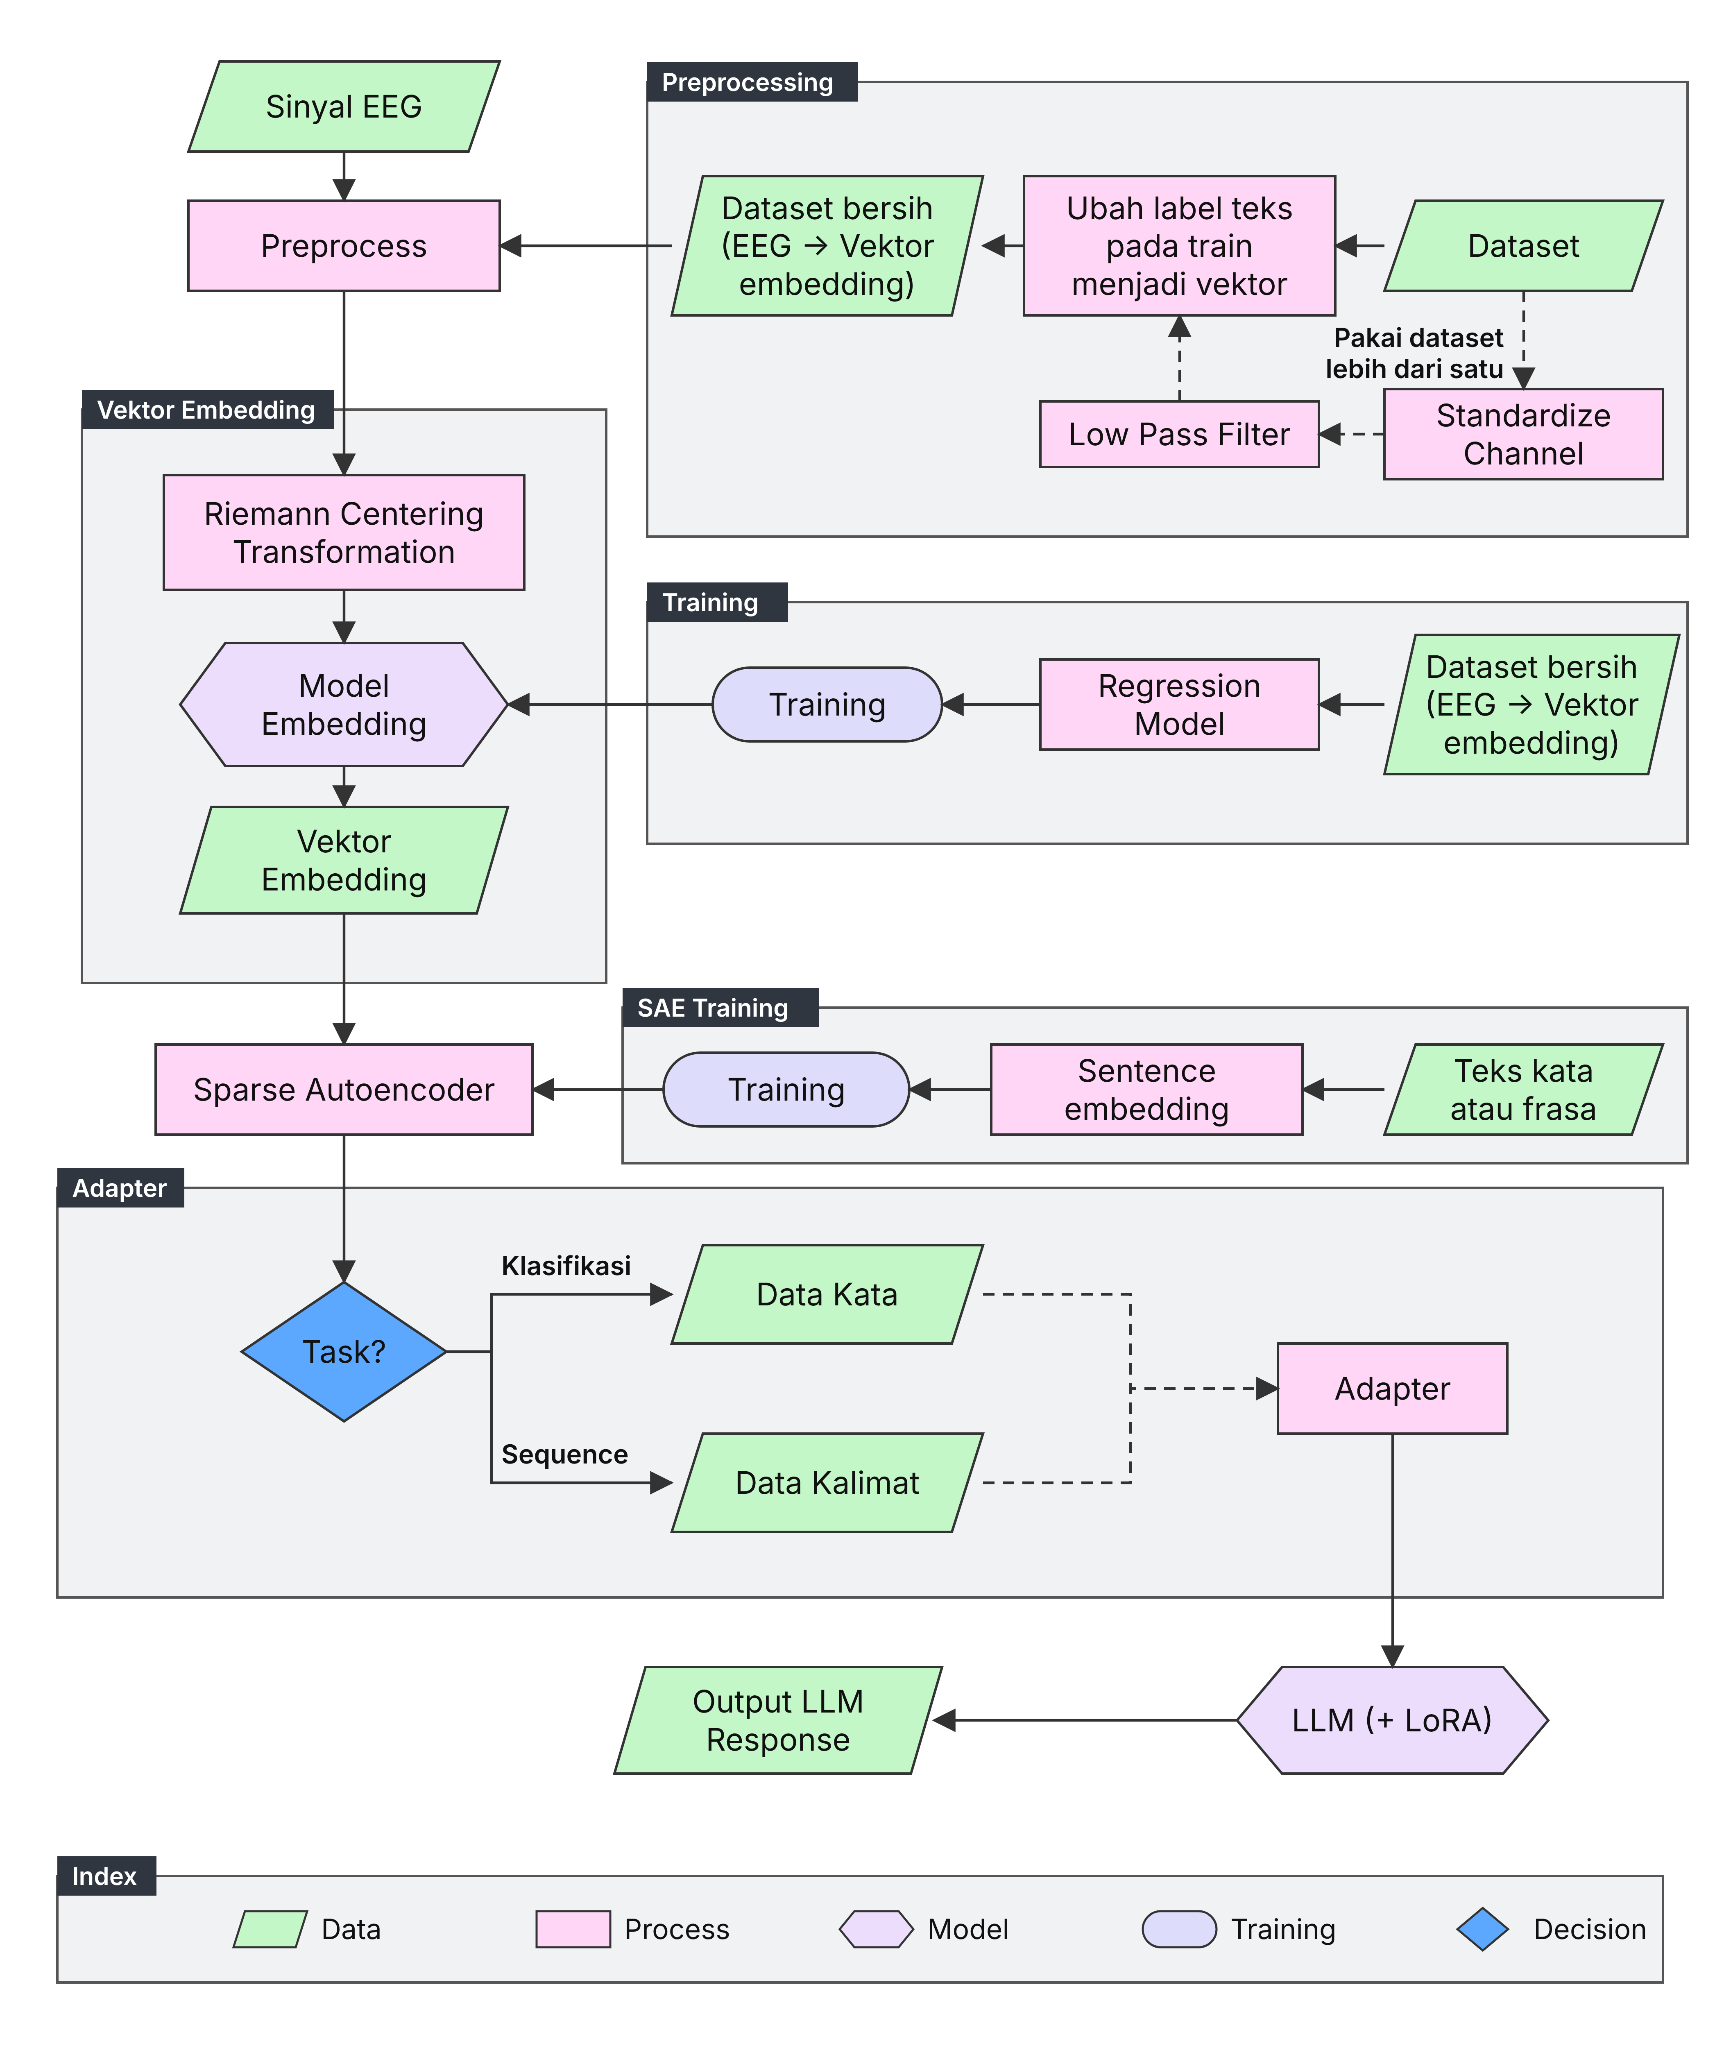
\includegraphics[width=0.9\textwidth]{images/gambar_IV_1_rancangan.png}
  \caption{Rancangan eksperimen dari sinyal EEG sampai keluaran LLM, beserta tahap prapemrosesan dan pelatihan model \textit{embedding}}
  \label{fig:rancangan}
\end{figure}

Alur utama ada pada kolom kiri Gambar~\ref{fig:rancangan} dan dibaca dari atas ke bawah.
Sinyal EEG dibersihkan pada tahap \textit{Preprocess}, diseragamkan antar subjek oleh \textit{Riemannian Centering Transformation} (RCT), lalu diubah oleh \textit{Model Embedding} menjadi vektor \textit{embedding}.
Vektor tersebut dipisahkan maknanya oleh \textit{Sparse Autoencoder} (SAE), diterjemahkan oleh \textit{Adapter} menjadi deretan vektor masukan LLM, dan akhirnya LLM yang dilengkapi LoRA menuliskan kata atau frasa yang dimaksud.

Tiga kotak di sebelah kanan menyiapkan alur utama.
Kotak \textit{Preprocessing} menyiapkan \textit{dataset}, yaitu membersihkan sinyal dan mengubah label teks pada data latih menjadi vektor, lalu hasilnya diteruskan ke tahap \textit{Preprocess}.
Kotak \textit{Training} melatih model regresi yang kemudian menjadi \textit{Model Embedding} pada alur utama.
Kotak \textit{SAE Training} melatih SAE dari teks kata atau frasa.
Kotak \textit{Adapter} di bagian bawah memuat keputusan tentang data teks apa yang dipakai untuk melatih \textit{adapter}.
Garis putus-putus menunjukkan jalur yang hanya dijalankan pada kondisi tertentu.

RCT dan SAE dapat dilewati.
Bila dilewati, masukan tahap tersebut langsung diteruskan ke tahap berikutnya.
Dengan cara ini, pengaruh RCT dan SAE dapat diuji satu per satu dari rancangan yang sama, yaitu dengan menjalankannya dengan dan tanpa masing-masing komponen.

% ============================================================================================
% IV.2 Perbandingan
% ============================================================================================
\section{Perbandingan dengan Eksperimen yang Ada Saat Ini}
\label{sec:perbandingan}
Sebagai pembanding dipakai Thought2Text \parencite[lihat Subbab~\ref{sec:penelitian-terkait}]{mishra2025}, karena alurnya dekat dengan rancangan ini di antara penelitian yang ditelaah.
Keduanya mengubah sinyal EEG menjadi vektor, menerjemahkan vektor itu ke ruang masukan LLM, lalu membiarkan LLM menuliskan teks.
Perbedaannya dengan rancangan ini dirangkum pada Tabel~\ref{tab:perbandingan}.

\begin{table}[t]
  \centering
  \caption{Perbandingan eksperimen yang ada saat ini (\textit{before}) dengan rancangan eksperimen ini (\textit{after})}
  \label{tab:perbandingan}
  \footnotesize
  \begin{tabularx}{\textwidth}{| Z{0.17\textwidth} | Y | Y |}
    \hline
    Aspek & Eksperimen saat ini (Thought2Text) & Rancangan eksperimen ini \\
    \hline
    Sinyal & EEG saat subjek melihat gambar, enam subjek, 128 \textit{channel} & EEG saat subjek membayangkan satu kata atau frasa (\textit{imagined speech}) \\
    \hline
    Prapemrosesan & \textit{Band-pass} 55 sampai 95 Hz dan \textit{notch} 50 Hz & Penyaringan frekuensi dan pembuangan \textit{noise}, serta pengubahan label teks data latih menjadi vektor 384 dimensi \\
    \hline
    Penyeragaman antar subjek & Tidak ada & RCT pada setiap subjek, dapat dilewati \\
    \hline
    Pengujian antar subjek & Evaluasi utama menggabungkan enam subjek, analisis per subjek melatih dan menguji model pada subjek yang sama & Pengujian per subjek dan lintas subjek, yaitu diuji pada subjek yang tidak dipakai saat pelatihan \\
    \hline
    Vektor dari sinyal & \textit{Encoder} EEG dilatih mendekati \textit{embedding} gambar CLIP (512 dimensi) & Model regresi dari fitur EEG ke \textit{embedding} teks label (384 dimensi) \\
    \hline
    Pemisahan makna pada vektor & Tidak ada & SAE, dapat dilewati \\
    \hline
    \textit{Adapter} & Satu lapis linear (\textit{projector}) & MLP yang menghasilkan $K$ vektor berukuran 4096, dengan $K$ ditentukan melalui \textit{tuning} \\
    \hline
    Penyesuaian LLM & LLM dibekukan, hanya \textit{adapter} yang dilatih & LLM dibekukan, LoRA ditambahkan bila \textit{adapter} saja belum cukup \\
    \hline
    Keluaran & Satu kalimat deskripsi gambar & Satu kata atau frasa, atau deretan kata \\
    \hline
    Penilaian & BLEU, METEOR, ROUGE, BERTScore, dan penilaian GPT-4 & \textit{Balanced accuracy} untuk kata, BERTScore \textit{recall} untuk deretan kata \\
    \hline
  \end{tabularx}
\end{table}

Thought2Text memakai EEG yang muncul saat melihat gambar, sedangkan rancangan ini memakai \textit{imagined speech}, yaitu sinyal tanpa rangsangan dari luar.
Karena tugas keduanya berbeda, bagian ini membandingkan rancangannya, dan perbandingan performa dengan BERTScore sebagai metrik yang sama dilakukan pada pengujian di Bab~\ref{chap:rencana-selanjutnya}.

Thought2Text tidak memuat penyeragaman sinyal antar subjek, dan penulisnya menyarankan metode yang meningkatkan generalisasi antar subjek \parencite{mishra2025}.
Rancangan ini menambahkan RCT dan menguji pengaruhnya pada pengujian lintas subjek (P04).
Dari sisi vektor, Thought2Text mendekatkan sinyal ke \textit{embedding} gambar, sedangkan rancangan ini mendekatkannya ke \textit{embedding} teks dari label (P02).
Vektor itu dapat dipisahkan maknanya dengan SAE (P05), lalu \textit{adapter} menerjemahkannya menjadi $K$ vektor masukan LLM, dengan LoRA bila diperlukan (P03).

Keluaran Thought2Text berupa kalimat bebas yang dinilai dengan kemiripan teks.
Keluaran rancangan ini berupa kata atau frasa yang dinilai dengan \textit{balanced accuracy}, dan deretan kata yang dinilai dengan BERTScore \textit{recall}.
BERTScore dipakai di kedua eksperimen sehingga hasilnya dapat disandingkan.

% ============================================================================================
% IV.3 Rancangan tiap tahap
% ============================================================================================
\section{Rancangan Setiap Tahap}
\label{sec:rancangan-tahap}
Rancangan terdiri atas beberapa tahap sesuai urutan kerja pada Gambar~\ref{fig:rancangan}, yaitu prapemrosesan data, pelatihan model \textit{embedding}, pembentukan vektor \textit{embedding}, SAE, \textit{adapter}, serta LLM (+ LoRA) dan keluaran.
Pada prapemrosesan data, sinyal EEG disaring frekuensinya dan dibersihkan dari \textit{noise}, lalu label teks data latih diubah menjadi vektor makna.
Selanjutnya, pada pelatihan model \textit{embedding}, model regresi dilatih untuk memetakan fitur sinyal EEG ke vektor makna.
Pada pembentukan vektor \textit{embedding}, sinyal antar subjek diseragamkan dengan RCT, lalu model regresi tersebut mengubah sinyal menjadi vektor makna.
Vektor ini kemudian dipisahkan maknanya oleh SAE, diterjemahkan oleh \textit{adapter} menjadi $K$ vektor masukan LLM, dan terakhir LLM (+ LoRA) menuliskan kata atau frasa yang dimaksud.

\subsection{Prapemrosesan Data}
\label{sec:rancangan-prapemrosesan}
Tahap ini menyiapkan data sebelum dipakai model, ditunjukkan pada Gambar~\ref{fig:rancangan-prapemrosesan}.
Masukannya adalah \textit{dataset} berisi percobaan EEG \textit{imagined speech} beserta label teks berupa satu kata atau frasa.
Keluarannya adalah \textit{dataset} bersih berupa pasangan sinyal EEG dan vektor \textit{embedding} dari labelnya.
Pembagian data latih, validasi, dan uji mengikuti skema per subjek dan lintas subjek pada Bab~\ref{chap:analisis-masalah} dan Subbab~\ref{sec:validasi}, dan percobaan yang sama tidak boleh muncul di dua bagian sekaligus.

\begin{figure}[H]
  \centering
  % Tahap prapemrosesan (kotak Preprocessing pada Gambar IV.1), digambar ulang dengan label yang sama.
% Gaya bentuk dan warna ada di diagram_style.tex.
\begin{tikzpicture}[dgbase]
\hyphenpenalty=10000 \exhyphenpenalty=10000 % jangan memenggal kata di dalam node
\node[dgdata] (ds)  at (0,0)     {Dataset};
\node[dgproc, minimum width=3.0cm, text width=2.7cm] (ubah) at (7.4,0) {Ubah label teks pada train menjadi vektor};
\node[dgdata, minimum width=2.8cm, text width=2.0cm] (bersih) at (11.3,0) {Dataset bersih (EEG $\to$ Vektor \textit{embedding})};
\node[dgproc, minimum width=2.6cm, text width=2.3cm] (std) at (3.2,-2.6) {Standardize Channel};
\node[dgproc, minimum width=2.6cm, text width=2.3cm] (lpf) at (7.4,-2.6) {Low Pass Filter};

\draw[dgarr] (ds) -- (ubah);
\draw[dgarr] (ubah) -- (bersih);
\draw[dgdash] (ds.south) |- (std.west);
\draw[dgdash] (std) -- (lpf);
\draw[dgdash] (lpf.north) -- (ubah.south);
\node[dglabel, align=left, anchor=west] at ($(ds.south)+(0.12,-0.55)$) {Pakai dataset\\lebih dari satu};
\end{tikzpicture}

  \caption{Tahap prapemrosesan data (kotak \textit{Preprocessing} pada Gambar~\ref{fig:rancangan})}
  \label{fig:rancangan-prapemrosesan}
\end{figure}

Sinyal EEG disaring frekuensinya dan dibersihkan dari \textit{noise}, dan langkah yang sama dijalankan pada sinyal EEG baru pada kotak \textit{Preprocess} di alur utama.
Dengan demikian, sinyal saat pelatihan dan saat pengujian melewati perlakuan yang sama.
Gambar~\ref{fig:rancangan-prapemrosesan} menunjukkan langkah yang berkaitan dengan label teks dan dengan penyamaan antar rekaman.

Jalur utama pada gambar hanya memiliki satu langkah, yaitu mengubah label teks pada data latih menjadi vektor.
Langkah ini memakai model \textit{sentence embedding} all-MiniLM-L6-v2, yang menghasilkan satu vektor berukuran 384 untuk satu kata atau frasa.
Model \textit{sentence embedding} dipilih karena sebagian label berupa frasa, dan satu label tetap harus menjadi satu vektor \parencite{reimers2019}.
Label pada data uji tidak diubah, karena dipakai apa adanya untuk menilai kata keluaran LLM.

Jalur putus-putus dijalankan hanya bila jumlah \textit{channel} atau \textit{sampling rate} pada rekaman beragam, sedangkan model menerima masukan berukuran tetap.
Langkah \textit{Standardize Channel} memilih \textit{channel} yang dimiliki semua rekaman dan mengurutkannya dengan cara yang sama.
Langkah \textit{Low Pass Filter} membuang frekuensi tinggi sebelum \textit{sampling rate} disamakan ke nilai terendah di antara rekaman, agar tidak muncul \textit{aliasing}, yaitu frekuensi tinggi yang terbaca sebagai frekuensi rendah yang palsu \parencite{oppenheim2010}.
Frekuensi potongnya dipilih di bawah setengah \textit{sampling rate} tujuan.

\subsection{Pelatihan Model \textit{Embedding}}
\label{sec:rancangan-pelatihan}
Tahap ini melatih model yang memetakan sinyal EEG menjadi vektor makna berukuran 384, ditunjukkan pada Gambar~\ref{fig:rancangan-pelatihan}.
Masukannya adalah \textit{dataset} bersih dari tahap sebelumnya, dan keluarannya adalah model regresi yang dipakai sebagai \textit{Model Embedding} pada alur utama.

\begin{figure}[H]
  \centering
  % Tahap pelatihan model embedding (kotak Training pada Gambar IV.1), digambar ulang dengan label yang sama.
% Gaya bentuk dan warna ada di diagram_style.tex.
\begin{tikzpicture}[dgbase]
\hyphenpenalty=10000 \exhyphenpenalty=10000 % jangan memenggal kata di dalam node
\node[dgdata, minimum width=2.8cm, text width=2.0cm] (dts) at (0,0) {Dataset bersih (EEG $\to$ Vektor \textit{embedding})};
\node[dgproc, minimum width=2.6cm, text width=2.3cm] (reg) at (4.6,0) {Regression Model};
\node[dgtrain] (trn) at (8.9,0) {Training};

\draw[dgarr] (dts) -- (reg);
\draw[dgarr] (reg) -- (trn);
\draw[dgarr] (trn.south) -- ++(0,-0.9) node[below, font=\tiny\linespread{1}\selectfont, align=center] {ke \textit{Model Embedding}\\(alur utama)};
\end{tikzpicture}

  \caption{Tahap pelatihan model regresi (kotak \textit{Training} pada Gambar~\ref{fig:rancangan})}
  \label{fig:rancangan-pelatihan}
\end{figure}

Model memetakan fitur sinyal ke vektor makna dengan regresi, yaitu menghasilkan 384 angka penyusun vektor tersebut.
Model dilatih dengan meminimalkan selisih kuadrat antara vektor prediksi dan vektor target dari label, seperti pada Persamaan~\ref{eq:regresi}.
Jenis modelnya dipilih dari regresi linear sampai jaringan saraf kecil, dengan data validasi dipakai untuk memilih pengaturannya.

Fitur masukan model berasal dari matriks kovarians spasial setiap percobaan (Persamaan~\ref{eq:kovarians}), setelah dipusatkan oleh RCT bila RCT dipakai, lalu dipetakan ke \textit{tangent space} agar menjadi vektor \parencite{barachant2012}.
Data latih melewati RCT yang sama dengan alur utama, sehingga masukan model saat pelatihan dan saat pengujian berbentuk sama.
Pada pengujian lintas subjek, model hanya dilatih pada subjek selain subjek yang diuji.

\subsection{Pembentukan Vektor \textit{Embedding} dari Sinyal EEG}
\label{sec:rancangan-vektor}
Tahap ini mengubah sinyal EEG yang sudah bersih menjadi vektor \textit{embedding}, ditunjukkan pada Gambar~\ref{fig:rancangan-vektor}.
Tahap ini terdiri dari dua langkah, yaitu RCT dan \textit{Model Embedding}.

\begin{figure}[H]
  \centering
  % Tahap pembentukan vektor embedding dan masukan ke SAE (kotak Vektor Embedding dan Sparse Autoencoder
% pada Gambar IV.1), digambar ulang dengan label yang sama. Gaya ada di diagram_style.tex.
\begin{tikzpicture}[dgbase]
\hyphenpenalty=10000 \exhyphenpenalty=10000 % jangan memenggal kata di dalam node
\node[dgproc, minimum width=2.4cm, text width=2.15cm] (rct) at (0,0) {Riemannian Centering Transformation};
\node[dgmodel, minimum width=2.4cm] (mdl) at (3.4,0) {Model Embedding};
\node[dgdata, minimum width=2.2cm, text width=1.5cm] (vec) at (6.5,0) {Vektor Embedding};
\node[dgproc, minimum width=2.4cm, text width=2.1cm] (sae) at (9.6,0) {Sparse Autoencoder};

\begin{scope}[on background layer]
  \node[dggroup, fit=(rct)(mdl)(vec)] (grp) {};
\end{scope}
\node[dgtab] at (grp.north west) {Vektor Embedding};

\draw[dgarr] (rct) -- (mdl);
\draw[dgarr] (mdl) -- (vec);
\draw[dgarr] (vec) -- (sae);
\draw[dgarr] ($(grp.west)+(-0.9,0)$) -- (grp.west) node[pos=0, above, font=\tiny\linespread{1}\selectfont, align=center, xshift=0.4cm, yshift=0.05cm] {dari\\\textit{Preprocess}};
\draw[dgarr] ($(mdl.north)+(0,1.2)$) -- (mdl.north) node[pos=0, right, font=\tiny\linespread{1}\selectfont, xshift=0.05cm] {dari \textit{Training}};
\draw[dgarr] (sae.east) -- ++(0.8,0) node[pos=1, above, font=\tiny\linespread{1}\selectfont, xshift=-0.2cm] {ke \textit{Adapter}};
\end{tikzpicture}

  \caption{Tahap pembentukan vektor \textit{embedding} (kotak \textit{Vektor Embedding} pada Gambar~\ref{fig:rancangan}) dan masukannya ke SAE}
  \label{fig:rancangan-vektor}
\end{figure}

RCT dijalankan pada setiap subjek mengikuti Subbab~\ref{sec:rct}, yaitu menghitung matriks kovarians spasial setiap percobaan (Persamaan~\ref{eq:kovarians}), rata-rata Riemann (Persamaan~\ref{eq:rata-riemann}), lalu pemusatan matriks (Persamaan~\ref{eq:pemusatan}).
Untuk subjek yang diuji, rata-ratanya dihitung hanya dari rekaman subjek itu sendiri.
Bila RCT dilewati, matriks kovarians langsung dipetakan ke \textit{tangent space}.
\textit{Model Embedding}, yaitu model regresi hasil Subbab~\ref{sec:rancangan-pelatihan}, menerima fitur hasil tahap tersebut dan menghasilkan vektor \textit{embedding} berukuran 384.
Vektor ini diteruskan ke tahap berikutnya.

\subsection{\textit{Sparse Autoencoder}}
\label{sec:rancangan-sae}
\textit{Sparse Autoencoder} (SAE) bertujuan memisahkan makna yang tercampur pada vektor \textit{embedding}, karena satu dimensi pada vektor dapat aktif untuk beberapa makna yang tidak berhubungan \parencite{cunningham2023}.
SAE melebarkan vektor 384 dimensi menjadi vektor yang lebih lebar dengan hanya sedikit angka yang aktif, sehingga ciri yang tercampur menjadi lebih terpisah \parencite{bricken2023}.
Tahap ini ditunjukkan pada Gambar~\ref{fig:rancangan-sae}.

\begin{figure}[H]
  \centering
  % Tahap sparse autoencoder (kotak SAE Training dan Sparse Autoencoder pada Gambar IV.1), digambar ulang
% dengan label yang sama. Gaya bentuk dan warna ada di diagram_style.tex.
\begin{tikzpicture}[dgbase]
\hyphenpenalty=10000 \exhyphenpenalty=10000 % jangan memenggal kata di dalam node
\node[dgdata, minimum width=2.2cm, text width=1.5cm] (txt) at (0,0) {Teks kata atau frasa};
\node[dgproc, minimum width=2.4cm, text width=2.1cm] (emb) at (3.3,0) {\textit{Sentence embedding}};
\node[dgtrain] (trn) at (6.4,0) {\textit{Training}};
\node[dgproc, minimum width=2.4cm, text width=2.1cm] (sae) at (9.8,0) {Sparse Autoencoder};

\begin{scope}[on background layer]
  \node[dggroup, fit=(txt)(emb)(trn)] (grp) {};
\end{scope}
\node[dgtab] at (grp.north west) {SAE Training};

\draw[dgarr] (txt) -- (emb);
\draw[dgarr] (emb) -- (trn);
\draw[dgarr] (trn) -- (sae);
\draw[dgarr] ($(sae.north)+(0,1.2)$) -- (sae.north) node[pos=0, above, font=\tiny\linespread{1}\selectfont, align=center] {dari \textit{Vektor Embedding}};
\draw[dgarr] (sae.east) -- ++(0.8,0) node[pos=1, above, font=\tiny\linespread{1}\selectfont, xshift=-0.2cm] {ke \textit{Adapter}};
\end{tikzpicture}

  \caption{Tahap pelatihan dan penggunaan SAE (kotak \textit{SAE Training} dan \textit{Sparse Autoencoder} pada Gambar~\ref{fig:rancangan})}
  \label{fig:rancangan-sae}
\end{figure}

SAE dilatih terpisah dari data EEG dan tanpa label, memakai banyak \textit{embedding} teks dari model \textit{sentence embedding}.
Dengan cara ini, pelatihan SAE tidak bergantung pada jumlah data EEG, dan pada pengujian lintas subjek SAE tidak memakai data subjek yang diuji.
Setelah dilatih, SAE dibekukan dan hanya dipakai untuk memperbesar dimensi vektor hasil \textit{Model Embedding}.
Ukuran masukan \textit{adapter} mengikuti lebar SAE, tetapi bila SAE dilewati, vektor 384 dimensi langsung menjadi masukan \textit{adapter}.

\subsection{\textit{Adapter}}
\label{sec:rancangan-adapter}
\textit{Adapter} bertujuan menerjemahkan vektor dari ruang \textit{embedding} teks ke ruang masukan LLM, karena ukuran dan ruang kedua vektor berbeda, ditunjukkan pada Gambar~\ref{fig:rancangan-adapter}.
Vektor berukuran 384 tidak dapat langsung dibaca LLM yang menerima vektor berukuran lebih besar.

\begin{figure}[H]
  \centering
  % Tahap adapter, LLM, dan keluaran (kotak Adapter, LLM (+ LoRA), dan Output LLM Response pada Gambar IV.1),
% digambar ulang dengan label yang sama. Gaya ada di diagram_style.tex.
\begin{tikzpicture}[dgbase]
\hyphenpenalty=10000 \exhyphenpenalty=10000 % jangan memenggal kata di dalam node
\node[dgdec] (task) at (0,0) {Task?};
\node[dgdata, minimum width=2.2cm, text width=1.7cm] (kata)   at (2.9,1.35)  {Data Kata};
\node[dgdata, minimum width=2.2cm, text width=1.7cm] (kalimat) at (2.9,-1.35) {Data Kalimat};
\node[dgproc, minimum width=1.8cm, text width=1.5cm] (adp) at (5.5,0) {Adapter};
\node[dgmodel, minimum width=2.5cm, text width=2.0cm] (llm) at (8.5,0) {LLM (+ LoRA)};
\node[dgdata, minimum width=2.1cm, text width=1.4cm] (out) at (10.95,0) {Output LLM Response};

\begin{scope}[on background layer]
  \node[dggroup, fit=(task)(kata)(kalimat)(adp)] (grp) {};
\end{scope}
\node[dgtab] at (grp.north west) {Adapter};

% keputusan Task?
\draw[dgline] (task.east) -- ++(0.45,0) coordinate (pc);
\draw[dgarr] (pc) |- (kata.west) node[pos=0.25, left, dglabel] {Klasifikasi};
\draw[dgarr] (pc) |- (kalimat.west) node[pos=0.25, left, dglabel] {Sequence};
% data pelatihan adapter (garis putus-putus)
\draw[dgline, dashed] (kata.east) -| ($(adp.west)+(-0.4,0)$) coordinate (pj);
\draw[dgline, dashed] (kalimat.east) -| (pj);
\draw[dgdash] (pj) -- (adp.west);
% ke LLM dan keluaran
\draw[dgarr] (adp.east) -- (llm.west);
\draw[dgarr] (llm.east) -- (out.west);
% masukan dari SAE
\draw[dgarr] ($(grp.west)+(-0.7,0)$) -- (grp.west) node[pos=0, above, font=\tiny\linespread{1}\selectfont, xshift=0.25cm] {dari \textit{SAE}};
\end{tikzpicture}

  \caption{Tahap \textit{adapter}, LLM, dan keluaran (kotak \textit{Adapter} dan bagian kanan pada Gambar~\ref{fig:rancangan})}
  \label{fig:rancangan-adapter}
\end{figure}

\textit{Adapter} berupa MLP dengan satu lapis tersembunyi yang mengubah satu vektor masukan menjadi $K$ vektor berukuran 4096 \parencite[lihat Subbab~\ref{sec:adapter}]{mokady2021,qwen35}.
Nilai $K$ ditentukan melalui \textit{tuning} dengan data validasi, dengan $K = 10$ mengikuti ClipCap sebagai nilai awal.
Deretan $K$ vektor ini diletakkan di depan masukan LLM sebagai \textit{soft prompt} \parencite{lester2021}.

\textit{Adapter} dilatih dengan LLM yang dibekukan.
Untuk setiap percobaan latih, vektor hasil \textit{Model Embedding} diubah \textit{adapter} menjadi $K$ vektor, lalu LLM diminta menuliskan teks label percobaan itu.
Selisih antara teks yang dituliskan dan teks label dihitung dengan \textit{cross-entropy} pada \textit{token} label, lalu parameter \textit{adapter} diperbarui, beserta LoRA bila dipakai.

Keputusan \textit{Task?} pada gambar menentukan teks yang dipakai sebagai label saat melatih \textit{adapter}.
Pada jalur \textit{Klasifikasi}, label berupa kata atau frasa, sehingga keluaran LLM berupa kata atau frasa yang dinilai dengan \textit{balanced accuracy}.
Pada jalur \textit{Sequence}, label berupa kalimat, misalnya kalimat yang memuat kata tersebut, sehingga keluaran LLM berupa deretan kata yang dinilai dengan BERTScore \textit{recall}.
Pada kedua jalur, sinyal EEG berasal dari satu kata atau frasa.

\subsection{LLM dan LoRA beserta Keluaran}
\label{sec:rancangan-llm}
Tahap terakhir menuliskan kata atau frasa yang dimaksud, ditunjukkan pada bagian kanan Gambar~\ref{fig:rancangan-adapter}.
LLM yang dipakai adalah Qwen3.5-9B, model sumber terbuka dengan masukan berukuran 4096 dan 32 lapis \parencite[lihat Subbab~\ref{sec:qwen}]{qwen35}, yang dijalankan secara lokal.
LLM menerima $K$ vektor dari \textit{adapter} di depan perintah teks yang tetap, lalu menuliskan keluarannya \textit{token} demi \textit{token}.

Bobot LLM dibekukan.
LoRA ditambahkan di atas \textit{adapter} bila \textit{adapter} saja belum cukup, dengan matriks kecil yang dilatih pada setiap lapis Transformer seperti pada Persamaan~\ref{eq:lora} \parencite[lihat Subbab~\ref{sec:lora}]{hu2021}.
LoRA dilatih bersama \textit{adapter} dengan tujuan yang sama.

Keluaran LLM berupa teks, yaitu kata, frasa, atau deretan kata yang dituliskan.
Pada pengujian, keluaran berupa kata dinilai dengan \textit{balanced accuracy} terhadap label asli, dan keluaran berupa deretan kata dinilai dengan BERTScore \textit{recall} (lihat Subbab~\ref{sec:metrik}).

Sebagai pembanding, dijalankan dua metode pada data uji dan pembagian data yang sama.
Pembanding pertama adalah model klasifikasi yang memilih satu kata dari daftar kata target, memakai fitur masukan yang sama dengan model regresi.
Pembanding kedua adalah pencarian kata terdekat, yaitu vektor hasil \textit{Model Embedding} dicocokkan dengan vektor semua kata kandidat memakai \textit{cosine similarity} seperti pada Persamaan~\ref{eq:cosine}, dan kata dengan nilai tertinggi menjadi tebakan.
Kedua pembanding tidak melewati SAE, \textit{adapter}, dan LLM, dan dinilai dengan \textit{balanced accuracy} yang sama.
